\documentclass[a4paper]{article}
\usepackage{geometry}
\usepackage{graphicx}
\usepackage{hyperref}
\usepackage{amsmath}

\title{Weekly Challenge 12: K-edge Shortest Paths in Directed Graphs with Negative Weights}
\author{CS/CE 412/471 Algorithms: Design and Analysis}
\date{Spring 2025}

\begin{document}
\maketitle
\thispagestyle{empty}
\begin{center}
Total points: 30
\end{center}

\section*{Objective}
In this WC, you will work in groups and:
\begin{itemize}
    \item understand the basic algorithm/component/building block for various shortest path algorithms.
    \item demonstrate step-by-step working of the building block with examples and hand-drawn illustrations.
    \item implement the algorithm and verify correctness of your hand-crafted solutions.
\end{itemize}

\section*{The Problem}
Ashraf Courier Service is responsible for delivering urgent messages between cities. The king has decreed that messages should reach their destination as quickly as possible, but couriers can take at most two roads to complete their journey.

Some cities are directly connected by a road, while others require passing through an intermediate city. The time taken to travel along each road varies, and couriers must always choose the fastest possible route.

Your task is to help the Ashraf Courier Service determine the shortest possible delivery time between a source city and all other cities while ensuring that no courier ever takes more than two roads in a single trip.

\section*{Task 1 (10 points)}
For the graph shown in Figure \ref{fig:graph}, dry run Algorithm 1 shown in Figure \ref{fig:algo1} which finds at most 2-edge shortest distances from a source vertex a to all destination vertices k through intermediate vertices j. The source vertex would be S. You just need to submit \textbf{the final graph obtained after completing execution of the algorithm} as Figure \ref{fig:graph-task1}. Please make sure the positioning of the vertices remains the same, i.e., do not morph the graph, just modify weights or add new edges.

\section*{Task 2 (10 points)}
Implement Algorithm shown in Figure \ref{fig:algo1} and \textbf{visualize the resulting graph} using any graph visualization library. Include this image as Figure \ref{fig:graph-task2}. You may use any programming language of your choice. Additionally, \textbf{mention in the caption} of Figure \ref{fig:graph-task2} what the output graph will illustrate if we run Algorithm 1 on this resulting graph one more time.

\section*{Task 3 (10 points)}
Run Algorithm 1 for \textbf{\textit{p-1}} times, where p is the total number of vertices in the graph (i.e., p = 10), and \textbf{visualize the resulting graph} using any graph visualization library. Include this image as Figure \ref{fig:graph-task3}. Additionally, \textbf{mention in the caption} of Figure \ref{fig:graph-task3} what Algorithm 2 finds out.

\begin{figure}[h!]
    \centering
    \begin{minipage}{0.6\textwidth}
        \centering
        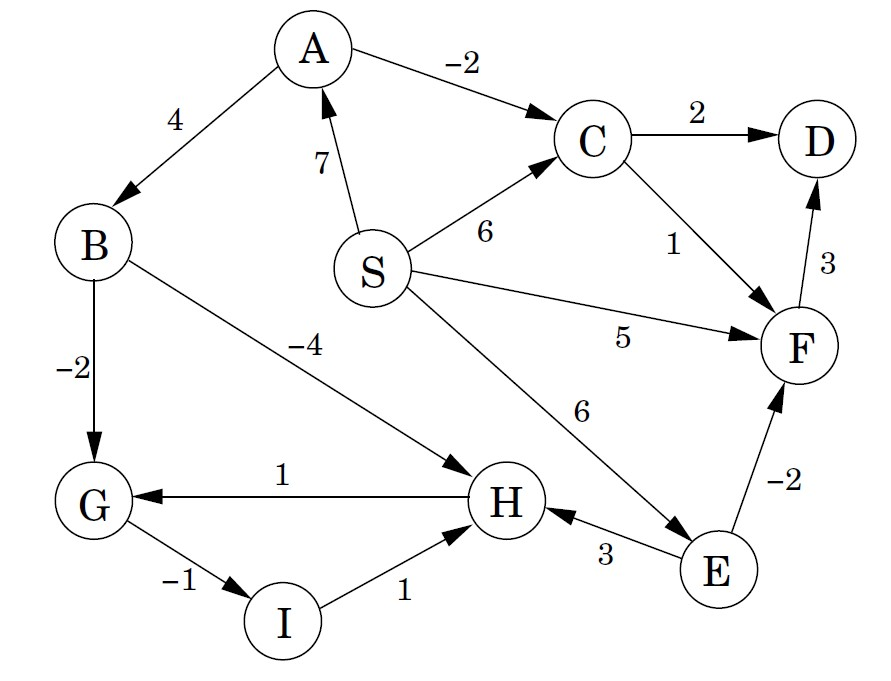
\includegraphics[width=\textwidth]{graph.jpg}
        \caption{The sample input graph}
        \label{fig:graph}
    \end{minipage}

    \vspace{1em} % Add vertical spacing

    \begin{minipage}{0.9\textwidth}
        \centering
        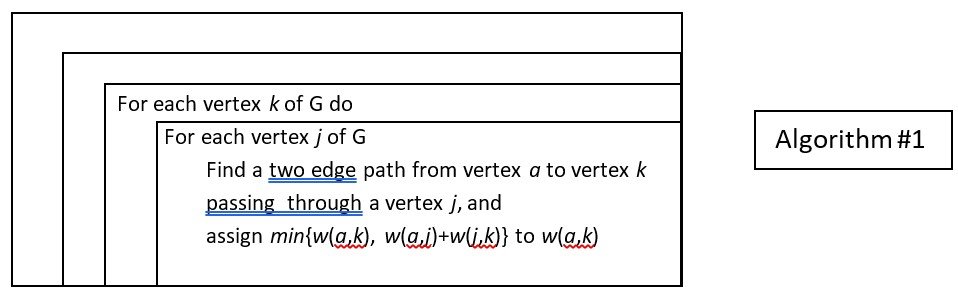
\includegraphics[width=\textwidth]{algo1.jpg}
        \caption{Algorithm 1 finds at-most 2-edge distances from a source vertex \textit{\textbf{a}} to all destinations \textbf{\textit{k}} through all intermediate nodes \textbf{\textit{j}}. w(a,k) refers to the weight of the edge $a\xrightarrow{}k$.}
        \label{fig:algo1}
    \end{minipage}

    \vspace{1em} % Add vertical spacing

    \begin{minipage}{0.9\textwidth}
        \centering
        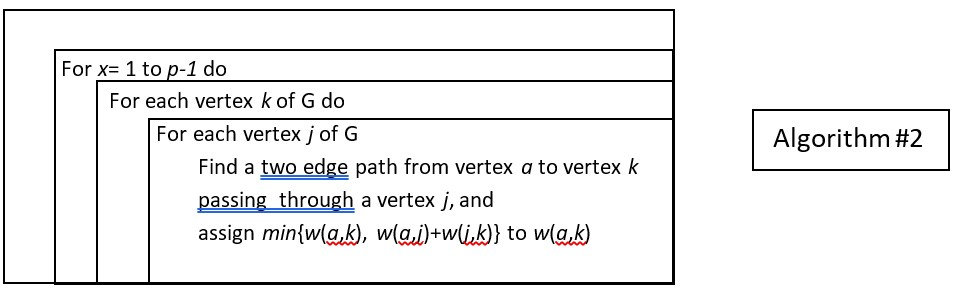
\includegraphics[width=\textwidth]{algo2.jpg}
        \caption{Algorithm 2 is designed by repeating Algorithm 1 (Figure \ref{fig:algo1}) \textbf{\textit{p-1}} times.}
        \label{fig:algo2}
    \end{minipage}
\end{figure}

\clearpage
\section*{Solution - Task 1 (Figure \ref{fig:graph-task1})}
\begin{figure}[h!]
    \centering
    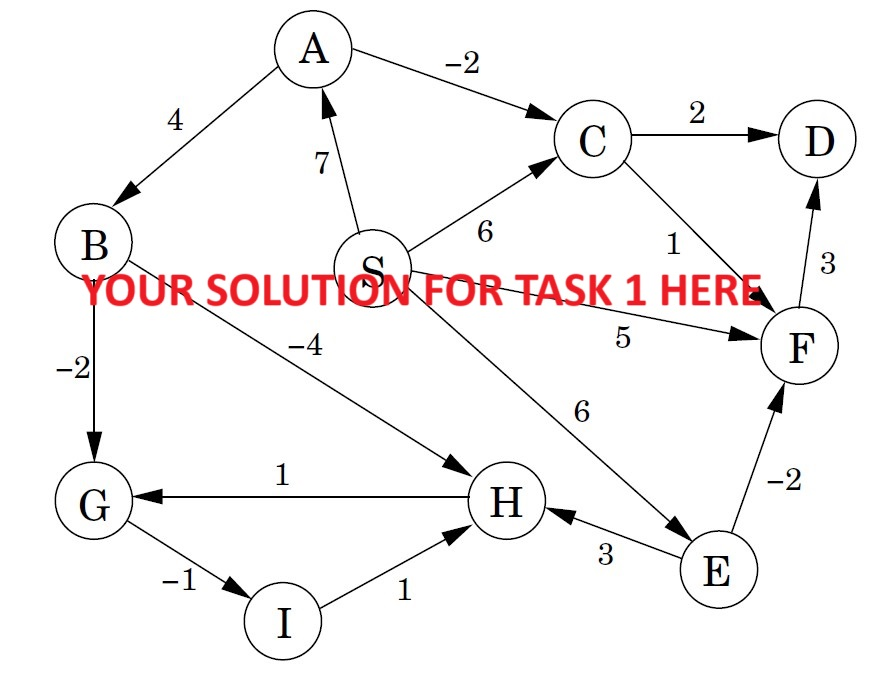
\includegraphics[width=0.6\textwidth]{graph-task1.jpg}
    \caption{Modified graph showing the at-most 2-edge shortest distances from source vertex S to all other vertices for the graph in Figure \ref{fig:graph}.}
    \label{fig:graph-task1}
\end{figure}

\clearpage
\section*{Solution - Task 2 (Figure \ref{fig:graph-task2})}
\begin{figure}[h!]
    \centering
    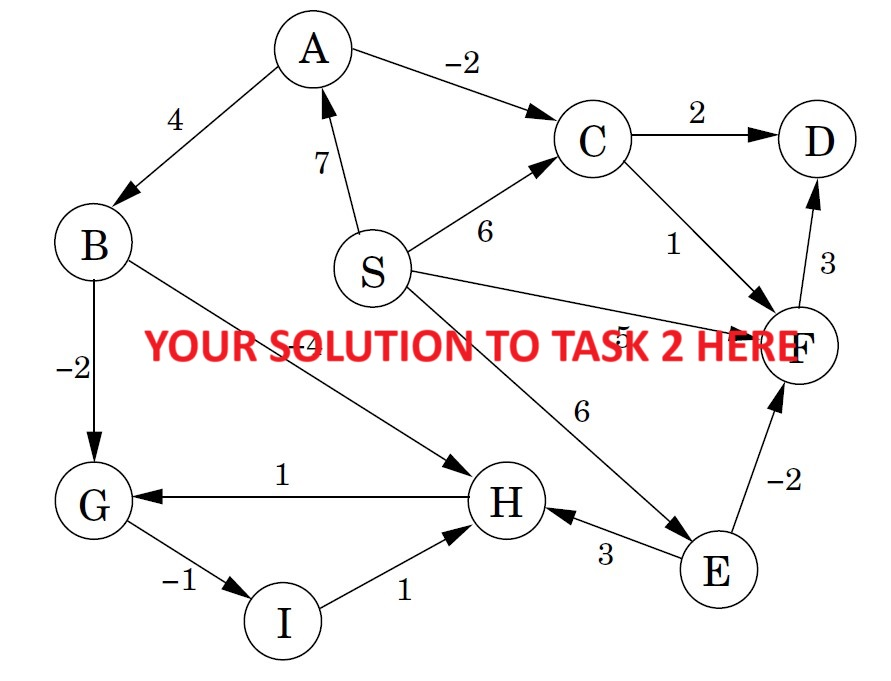
\includegraphics[width=0.6\textwidth]{graph-task2.jpg}
    \caption{Code-generated graph showing the at-most 2-edge shortest distances from source vertex S to all other vertices for the graph in Figure \ref{fig:graph}.}
    \label{fig:graph-task2}
\end{figure}

\clearpage
\section*{Solution - Task 3 (Figure \ref{fig:graph-task3})}
\begin{figure}[h!]
    \centering
    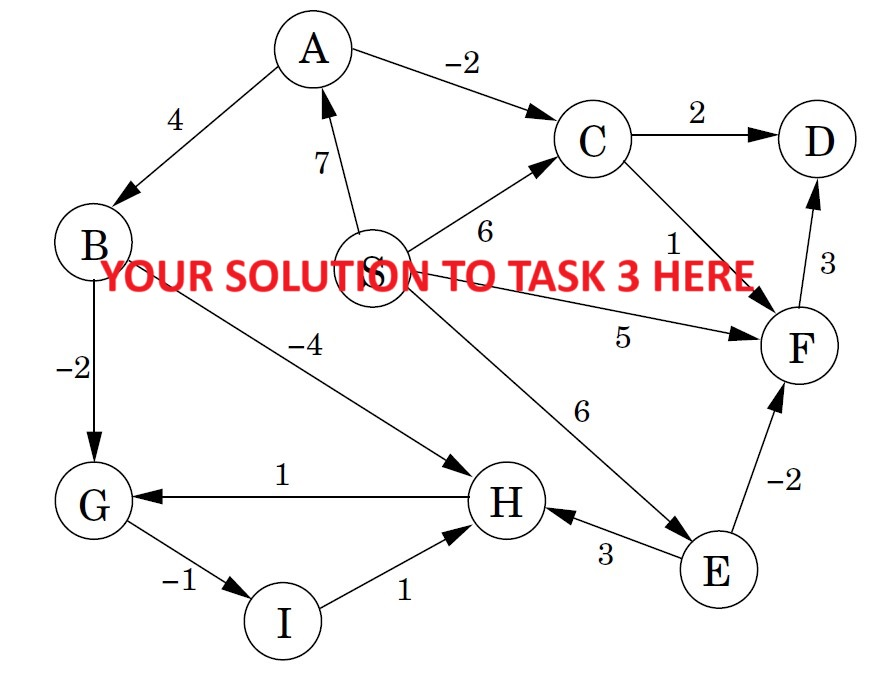
\includegraphics[width=0.65\textwidth]{graph-task3.jpg}
    \caption{Code-generated graph showing shortest distances from source vertex S to all other vertices for the graph in Figure \ref{fig:graph}.}
    \label{fig:graph-task3}
\end{figure}

\clearpage % Ensures all figures appear before the next section

\section*{Submission}
\begin{enumerate}
    \item Submit one PDF file including your solutions. 
    \item Submit one source file including your code. 
    \item Clearly write your group number, member names, and IDs. 
\end{enumerate}

\end{document}
